\documentclass[../main.tex]{subfiles}

\begin{document}

\section{Overwiew}
\label{section:problem:overview}
\begin{figure}[h]
    \centering
    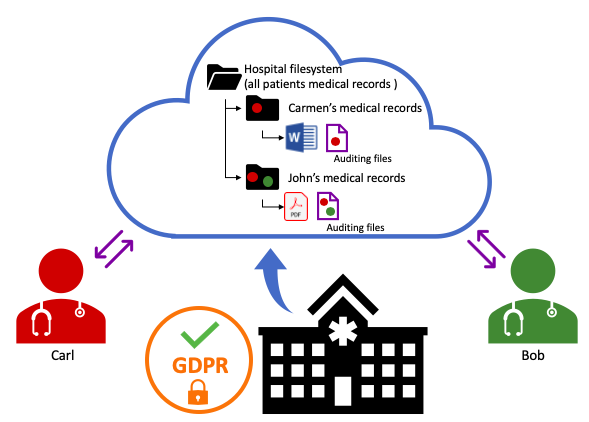
\includegraphics[width=0.75\textwidth]{../../images/problem/overview}
    
    \label{figure:problem:overview}
    \caption{Representation of the real life situation}
\end{figure}

\par As explained in the introduction, we are in a world were everything is being digitised and uploaded on remote storage. This raises an important question about data confidentiality: how can I use Cloud services while still being able to preserve confidential information against unauthorised parties, including the Cloud provider itself. Furthermore, how can we securely and efficiently share those information remotely stored without disclosing any secret to unauthorised parties.
\par A concrete and interesting application of this is linked to the healthcare domain, more precisely the hospitals. Inside an hospital, many services or doctors must share medical records of a single patient, as depicted in Figure \ref{figure:problem:overview}. How can those parties share this record without disclosing its content (to other parties) and without requiring complicated operation ? On top of that, the revocation of a doctor rights to access a specific resource, once he no longer needs it, is also a mandatory operation according GDPR.\\

\par Alongside data confidentiality, keeping track of who accessed or edited a given file is required. GDPR states that: "\textit{All EU institutions have the legal obligation to keep a central register of records of activities processing personal data}". In practice, this means that every time an authorised doctor wants to access a medical record, s/he must first explain its intention. As the intent may itself contain confidential information, it must also be securely stored. Most of all, these justification can not be tampered with, in order to keep their accuracy. Furthermore, for a forensic purpose, it would also be interesting to spot if unauthorised user are trying to alter these data. To top it all, these intents must be easily accessible for GDPR compliance evidence.

% healthcare regulation ????

\end{document} 